% Created 2011-12-09 Fri 03:13
\documentclass[bigger, english, 10pt, presentation]{beamer}
\usepackage[utf8]{inputenc}
\usepackage[T1]{fontenc}
\usepackage{fixltx2e}
\usepackage{graphicx}
\usepackage{longtable}
\usepackage{float}
\usepackage{wrapfig}
\usepackage{soul}
\usepackage{textcomp}
\usepackage{marvosym}
\usepackage{wasysym}
\usepackage{latexsym}
\usepackage{amssymb}
\usepackage{hyperref}
\tolerance=1000
\usepackage{loochao}
\providecommand{\alert}[1]{\textbf{#1}}

\title{Project Report}
\author{Chao LU\thanks{chaol@princeton.edu}}
\date{2011-12-09 Fri}

\begin{document}

\maketitle

\begin{frame}
\frametitle{Outline}
\setcounter{tocdepth}{3}
\tableofcontents
\end{frame}



\section{Microscopy Measurement}
\label{sec-1}
\subsection{Film Uniformity}
\label{sec-1-1}
\begin{frame}
\frametitle{10x lens}
\label{sec-1-1-1}
\begin{columns}
\begin{column}{0.5\textwidth}
%% A block
\label{sec-1-1-1-1}

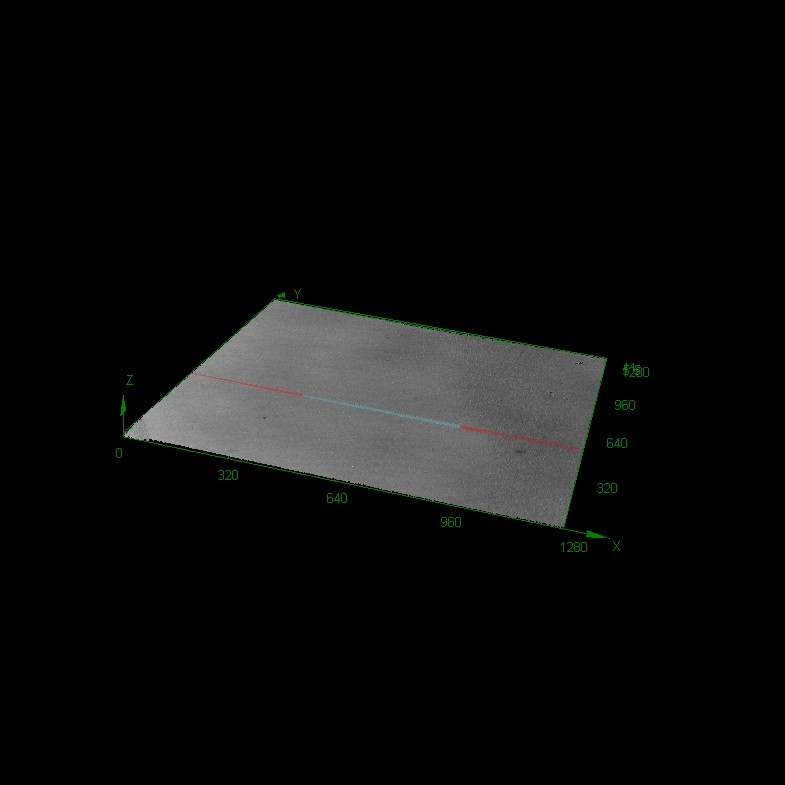
\includegraphics[width=.9\linewidth]{./figures/111208_As2S3_AsDep_UniformSite_10x_3D.jpeg}
\end{column}
\begin{column}{0.5\textwidth}
%% A block
\label{sec-1-1-1-2}

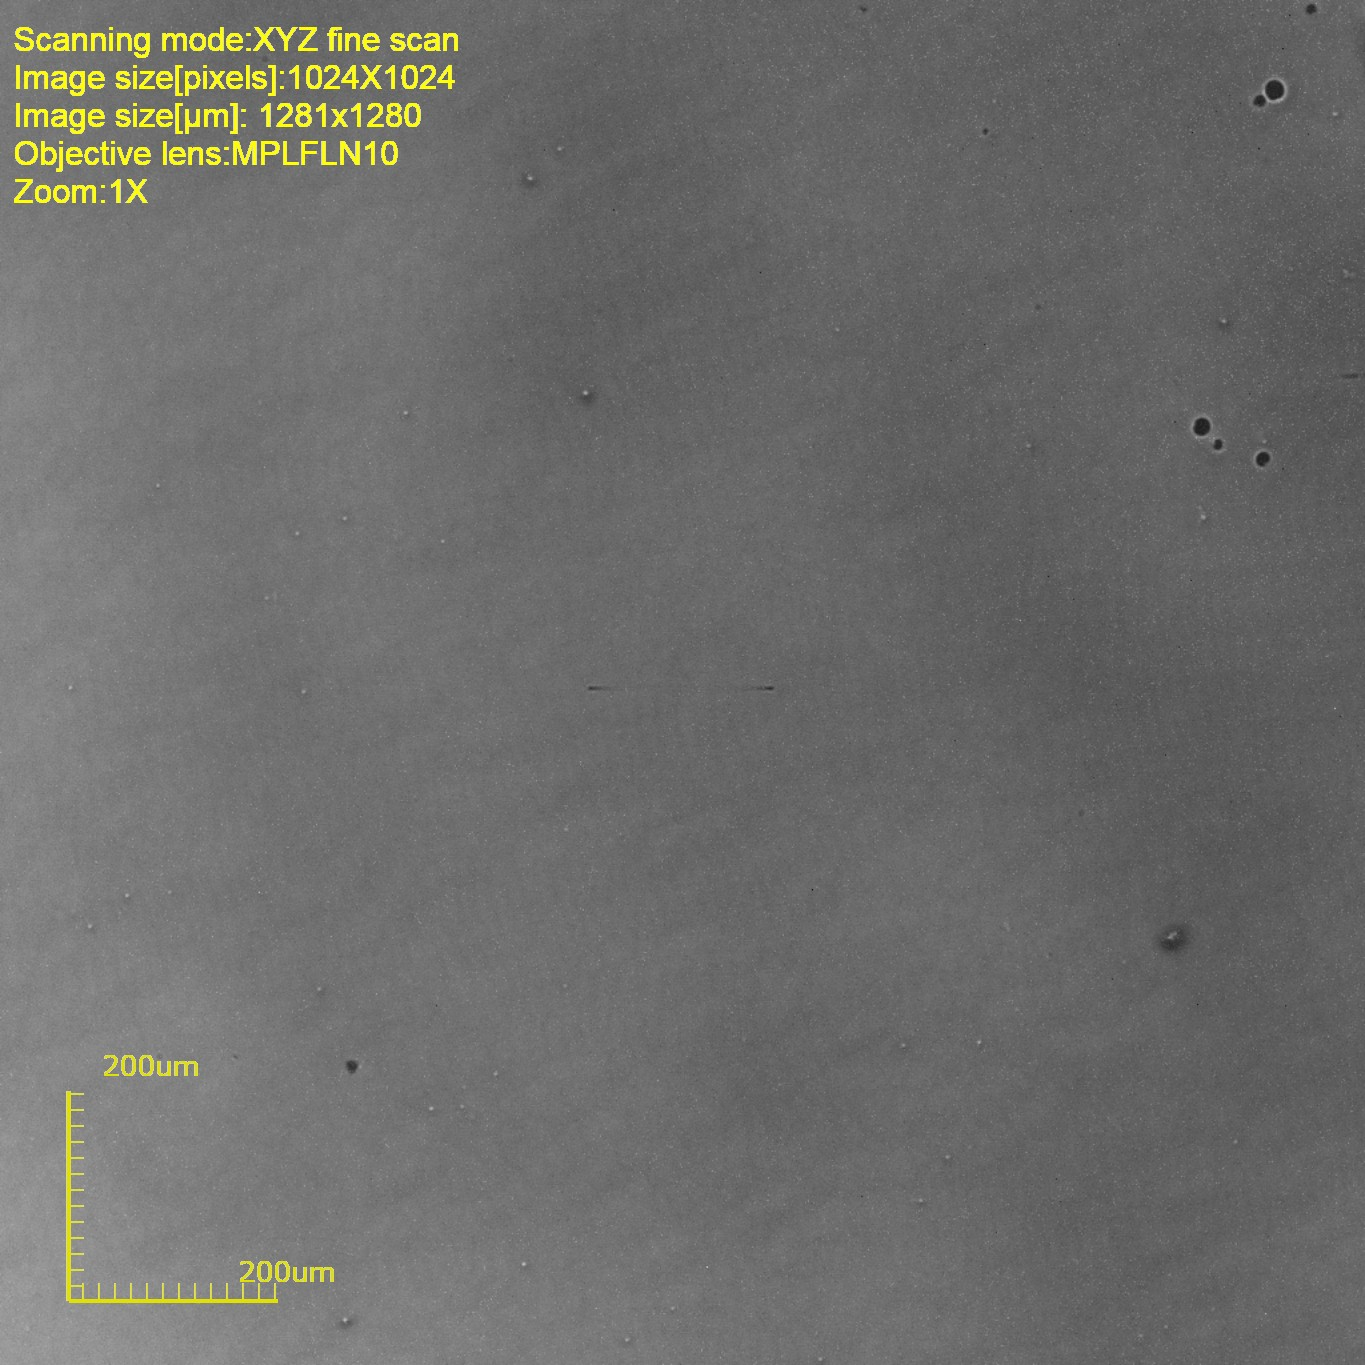
\includegraphics[width=.9\linewidth]{./figures/111208_As2S3_AsDep_UniformSite_10x_2D.jpeg}
\end{column}
\end{columns}
\end{frame}
\subsection{Film Thickness}
\label{sec-1-2}
\begin{frame}
\frametitle{Film Thickness}
\label{sec-1-2-1}
\begin{columns}
\begin{column}{0.7\textwidth}
%% A block
\label{sec-1-2-1-1}

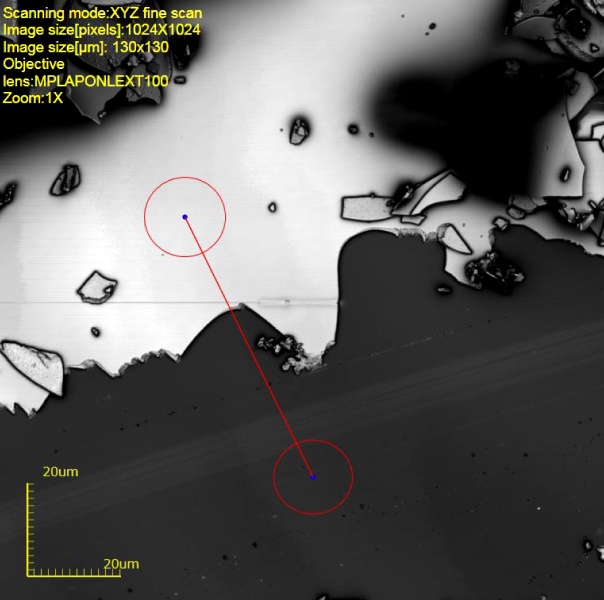
\includegraphics[width=.9\linewidth]{./figures/111208_As2S3_AsDeposited_100x_2D_HeightMeasurements.jpeg}
\end{column}
\begin{column}{0.3\textwidth}
%% A block
\label{sec-1-2-1-2}

\begin{itemize}
\item 0.747 $\mu m$
\item 100x lens
\end{itemize}
\end{column}
\end{columns}
\end{frame}
\section{Absorption Coefficient}
\label{sec-2}
\subsection{488nm and White Source}
\label{sec-2-1}
\begin{frame}
\frametitle{488nm and White Source}
\label{sec-2-1-1}
\begin{block}{488nm Measurements}
\label{sec-2-1-1-1}

\begin{itemize}
\item W/O film: 17.82W
\item With film: 17.82W
\item The film is too thin to absorb much, maybe good for us?
\end{itemize}
\end{block}
\begin{block}{TODO}
\label{sec-2-1-1-2}

\begin{itemize}
\item Add ND filter and retest.
\item Increase the film thickness.
\item How to increase thickness to upto $200 \mu m$???
\end{itemize}
\end{block}
\begin{block}{White source}
\label{sec-2-1-1-3}

\begin{itemize}
\item Tried last night.
\item May need Maike's help: Mounts and driver for the spectrometer.
\end{itemize}
\end{block}
\end{frame}
\section{Refractive index}
\label{sec-3}
\subsection{Refractive index}
\label{sec-3-1}
\begin{frame}
\frametitle{Refractive index}
\label{sec-3-1-1}
\begin{block}{dn/dt}
\label{sec-3-1-1-1}

\begin{itemize}
\item Cooling system needed if we want data for long time like 2hours.
\item Black enclosure needed as well.
\item Film ready for 20min, need to test $\Delta n$, thanks for Jerry's help
\end{itemize}
\end{block}
\begin{block}{dn/dx}
\label{sec-3-1-1-2}

\begin{itemize}
\item How to focus tight. Now it's mm.
\item How to measure spot size.
\item How to measure such small changes, Raman?
\item How to mark this spot size out.
\end{itemize}
\end{block}
\end{frame}
\section{TODO}
\label{sec-4}
\subsection{TODO}
\label{sec-4-1}
\begin{frame}
\frametitle{TODO}
\label{sec-4-1-1}
\begin{block}{TODO List}
\label{sec-4-1-1-1}

\begin{itemize}
\item Mechanism of hologram, like multiplexing.
\item How to fabricate thick film, where are we now?
\item OptiGrate.
\item FTIR -- Maike?
\end{itemize}
\end{block}
\end{frame}

\end{document}